\documentclass[11pt,a4paper]{extarticle}
\usepackage{cmap}
\usepackage[utf8x]{inputenc}
\usepackage[T2A,T1]{fontenc}
\usepackage[hidelinks]{hyperref} 
\usepackage[russian,english]{babel}
\usepackage{listings,lstautogobble}
\usepackage{amsthm}
\usepackage{amsmath}
\usepackage{amsfonts}
\usepackage{amssymb}
\usepackage{cite}
\usepackage{xcolor,colortbl}
\usepackage{graphicx}
\usepackage{mathtools}
\usepackage{subcaption}
\usepackage{enumerate}
\usepackage{perpage}
\usepackage{subcaption}
\usepackage{fullpage}
\usepackage[nottoc,numbib]{tocbibind}
\usepackage[russian,english]{babel}

\definecolor{Gray}{gray}{0.95}
\definecolor{Red}{rgb}{0.80,0.5,0.5}
\definecolor{Green}{rgb}{0.6,0.8,0.6}

\definecolor{Gray}{gray}{0.95}
\definecolor{Black}{gray}{0.1}
\definecolor{Red}{rgb}{0.80,0.5,0.5}
\definecolor{Green}{rgb}{0.6,0.8,0.6}

\definecolor{codegray}{rgb}{0.5,0.5,0.5}
\definecolor{codepurple}{rgb}{0.58,0,0.82}
\definecolor{backcolour}{rgb}{0.95,0.95,0.92}

\newlength{\twosubht}
\newsavebox{\twosubbox}
\setlength\headheight{26pt}

\lstdefinestyle{codestyle}{
    backgroundcolor=\color{backcolour},   
    commentstyle=\color{Green},
    breakatwhitespace=false,         
    breaklines=true,                 
    captionpos=b,                    
    keepspaces=true,                 
    showspaces=false,                
    showstringspaces=false,
    showtabs=false,                  
    tabsize=2,
    autogobble=true,
    inputencoding=utf8x,
    extendedchars=\true
}

\lstset{style=codestyle}

\newenvironment{compactlist}{
\begin{list}{{$\bullet$}}{
\setlength\partopsep{0pt}
\setlength\parskip{0pt}
\setlength\parsep{0pt}
\setlength\topsep{0pt}
\setlength\itemsep{0pt}
}}{
\end{list}
}

\MakePerPage{footnote}


\begin{document}
\selectlanguage{russian}
\begin{titlepage}
	\begin{centering}
		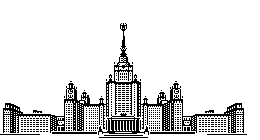
\includegraphics{img/msu}\\
		\large{
			\textbf{Московский государственный университет имени М.В. Ломоносова}\\
			Факультет вычислительной математики и кибернетики\\
			Кафедра интеллектуальных информационных технологий\\
			Лаборатория компьютерной графики и мультимедиа\\[4cm]
		}
		\Large{
			Гончаренко Дмитрий Александрович\\[0.9cm]
		}
		\Large{
			\textbf{Алгоритм изменения времени суток на изображении}\\
			% \textbf{Research of Changing The Time of Day on Images}\\
		}
		\rule[0.3cm]{14cm}{0.02cm}\\[1cm]
		\large{
			ВЫПУСКНАЯ КВАЛИФИКАЦИОННАЯ РАБОТА\\[4cm]
		}
	\end{centering}
	\begin{flushright}
		\large{
			\textbf{Научный руководитель:}\\ К.С. Зипа\\
		}
	\end{flushright}
	\begin{center}
		\vfill
		\large{
			Москва, 2019
		}
	\end{center}
\end{titlepage}

\begin{abstract}
	Алгоритм изменения времени суток на изображении относится к классу задач машинного обучения по \textit{переносу
	изображений}\footnote{
		\textbf{Перенос изображений} (англ. \textit{image translation}, или \textit{image transfering})
		-- подвид технологии переноса обучения, позволяющий сохранять и объединять локальные признаки изображений.
	}.
	Данная сфера значительное продвинулась благодаря современным вычислительным возможностям, в частности переносе обучения на графические процессоры, GPU.
	За последние несколько лет появилось немало исследовательских работ на тему переноса изображений, стилей и колоризации.
	В данной работе рассматриваются современные подходы к переносу изображений, применимые к задаче изменения времени суток на изображении.
	Проводится описание нейросетевых моделей, обоснование и выбор метода для обучения и сравнительный анализ серии экспериментов обучения.
\end{abstract}

\selectlanguage{english}
\begin{abstract}
	The algorithm of changing the time of the day on images is a subclass of Machine Learning problems of image translation.
	This area has advanced significantly due to the modern computing capabilities, in particular the training transfer on GPUs.
	Over the past few years, many research papers have appeared on the subjects of images translation, styles transfering and colorization.
	This research reveals modern approaches of image translation applicable to problem of changing the time of day on the image.
	A description of the neural network models, the rationale and choice of method for training, and a comparative quality analysis of a series of training experiments are carried out.
\end{abstract}
\selectlanguage{russian}

\newpage
\tableofcontents
\newpage

\section{Введение}
	Математические описания моделей машинного обучения появились еще в середине 20-го века.
	А первые попытки их практической реализации начались в конце 50х годов.
	Спустя полвека задачи машинного обучения все также не теряют своей актуальности.
	Рост числа работ, открытие исследовательских центров внутри компаний и при университетах показывает,
	что высокий интерес к данной сфере не ограничивается только наукой.
	За последние 10 лет появилось множество удобных инструментов для построения самых разнообразных моделей обучения, что оказало немалое влияние на развитие \textit{науки о данных}\footnote{
		\textbf{Наука о данных} (англ. \textit{data science}) -- соовокупность процессов и методов направленных на извлечение информации из исследуемых данных.
	}.  
	
	Стоит отметить, что не последнюю роль здесь сыграли многократно выросшие вычислительные возможности. 
	Это позволило обучать \textit{нейронные сети}\footnote{
		\textbf{Нейронная сеть} --  математическая модель, а также её программное или аппаратное воплощение, 
		построенная по принципу организации и функционирования биологических нейронных сетей -- сетей нервных клеток живого организма.
		Является мощным современным инструментом машинного обучения.
		Главная особенность -- способность обучаться на предоставленных данных, называемых тренировочными.
		Помимо исследовательских направлений нейронные сети также активно используются в комерции, например обработка спама на электронной почте или система рекомендаций в интернет-магазинах.
	} на персональных компьютерах за доли секунды, для чего ранее могли требоваться дни, а то и недели на специализированных вычислительных устройствах.

	\textit{Перенос обучения} является одной из центральных исследовательских задач современного машинного обучения.
	Данная область направленна на получение некоторой информации об объекте, сохранение и последующее применение этих знаний к другому объекту, связанному с первым.   
	\textit{Перенос изображений}, в свою очередь, является подклассом переноса обучения применяемым на изображениях. 
	В настоящее время переносу изображений уделяется значительное внимание в исследовательских работах \cite{i2ipapers}, а разнообразие сферы применения поистине впечатляющее.
	Так с помощью переноса изображений можно добиться объединения стилей двух изображений \cite{style_transfer}, что может использоваться художниками в создании интересных картин и композиций,
	колоризации\footnote{ \textbf{Колоризация} (англ. \textit{colorization}) -- преобразование монохромных изображений в цветные.} черно-белых фотографий \cite{color_transfer},
	благодаря чему можно в автоматизированном режиме перекрашивать отцифрованные монохромные киноленты и фотоснимки,
	объединение локальных признаков объектов и животных \cite{CycleGAN}, что позволяет создавать несуществующие породы животных и по наброску генерировать текстурированное изображение,
	увеличение разрешения изображений \cite{super_resolution}, с помощью чего можно достигать точности, превышающей традиционные алгоритмы билинейной интерполяции.

	В данной исследовательской работе рассматриваются и систематизируются современные подходы переноса изображений, применимые к задаче изменения времени суток на изображениях.
	Проводится обучение подходящего алгоритма на различных наборах тренировочных данных.
	Моя задача состоит в получении предобученной модели, умеющей из изображений дня синтезировать реалистичные изображения ночи,
	и наоборот из ночи научиться генерировать максимально правдоподобное изображение дня. 
	Также я провожу сравнительный анализ скорости переноса и качества полученных результатов.
	
	В качестве инструмента был выбран фреймворк PyTorch\footnote{
		\textbf{PyTorch} -- библиотека машинного обучения, основанная на Torch. Разработана исследовательской группой в Facebook.
	}, так как он разработан в виде библиотеки для языка Python -- основного языка современного машинного обучения \cite{ml_lang},
	и зарекомендовал себя мощным и гибким инструментом для исследования и обучения нейронных сетей.

\newpage
\section{Постановка задачи}
	% \subsection{Актуальность задачи}
	% 	Решение задачи изменения времени суток можно использовать при создании 3D моделей и макетов,
	% 	не будет необходимости перирисовывать и видоизменять модель для ночной сцены, если уже создана дневная.
	% 	для видеоиграх, для смены времени сцены, в рекламе.

	\subsection{Цель работы}
		В науке о данных одну из ключевых ролей играет непосредственный выбор данных, на которых будет обучаться сеть, 
		и которые будут использоваться для валидации качества модели. Перенос изображений не является исключением.
		Цель работы -- получить модель, которая будет уметь переносить изображения между \textit{доменами}\footnote{
			\textbf{Домен} -- область, множество, содержащее в себе объекты одного типа. 
		} дня и ночи и будет способна с высокой точностью решить проблему изменения времени суток на изображениях.

	\subsection{Решаемые задачи}
		Проблему изменения времени суток на изображении можно разбить на следующие этапы:

		\begin{compactlist}
			\item Исследование существующих методов переноса изображений и анализ решений родственных задач
			\item Поиск применимых к проблеме тренировочных данных -- изображений с различными временем суток
			\item Классификация тренировочных данных и перенос изображений по доменам 
			\item На основе проведенного исследования и обзора литературы, выбор модели, подходящей для решения поставленной задачи
			наилучшим образом
			\item Множественное обучение выбранной модели с различными конфигурациями на наборах данных с помощью библиотеки PyTorch
			\item Проведение серии экспериментов переноса изображений для получения оценки качества и скорости работы модели 
		\end{compactlist}

	\subsection{Формальная постановка задачи}\label{intro_problem}
		Формально алгоритм изменения времени суток на изображении можно сформулировать следующим образом:
		\vspace{-1em}
		\subsubsection*{Вход}
			На вход алгоритму поступают два изображения из различных доменов \(x_{1} \in X_{1}\)  и \(x_{2}\ \in X_{2}\), где
			\begin{itemize}
				\item \(X_{1}\) -- домен с набором изображений первого типа
				\item \(X_{2}\) -- домен с набором изображений второго типа
			\end{itemize}
			Не ограничивая общности, пусть \(X_{1}\) соодержит изображения дня, а \(X_{2}\) соответвует ночи.
		\vspace{-1em}
		\subsubsection*{Выход}
			Необходимо построить \textit{кросдоменные}\footnote{
				\textbf{Кросдоменный перенос} (англ. \textit{cross-domain transfer}) -- перенос объектов между доменами 
			} отображения \(f_{12}\!: X_{1} \longrightarrow X_{2}\) и \(f_{21}\!: X_{2} \longrightarrow X_{1}\).
			
			\noindent
			Реализовать функцию, принимающую на вход изображения из разных доменов
			\(x_{1}, x_{2}\) и возвращающую перенесенные изображения \(x_{2}', x_{1}'\) соответсвенно: 

			\begin{equation}
					x_{2}', x_{1}'  = CrossDomainTranslator(x_{1}, x_{2}),\ \text{где}\ x_{1}' \in X_{1},\ x_{2}' \in X_{2}
			\end{equation}
	
	\newpage
	\section{Обзор существующих методов}
		
		Одними из наиболее популярных алгоритмов, на которых базируются решения многих задач переноса изображений, на сегодняшний день являются
		генеративно состязательные нейронные сети и вариационные автоэнкодеры.

		\subsection{Генеративно состязательные сети (GAN)}		

			\textbf{Генеративно состязательная нейронная сеть} (GAN) -- комбинация двух нейронных сетей $G$ (генератор) и $D$ (дискриминатор).
			Генератор подбирает \textit{латентные}\footnote{
				\textbf{Латентный} здесь и далее, то же что и скрытый
			} параметры для генерации нового объекта.
			Дискриминатор пытается отличить оригинал от объекта, созданного генератором.
			
			\begin{figure}[ht]
				\centering
				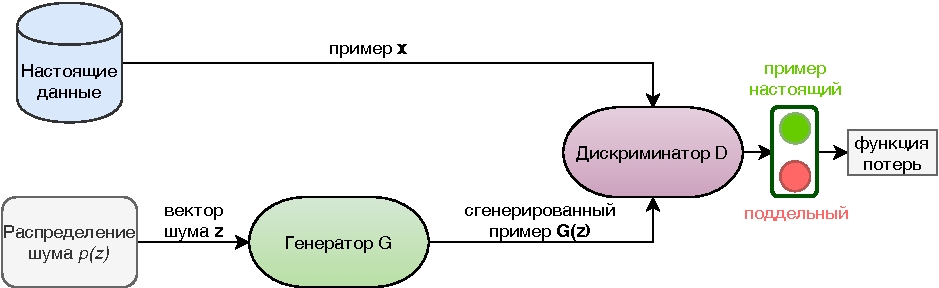
\includegraphics[width=0.8\textwidth]{img/gan}
				\caption{Схема работы генеративно состязательной сети (GAN)}
				\label{fig:gan}
			\end{figure}
			\noindent
			Формально генератор можно определить как отображение некоторого пространства скрытых параметров $\mathcal{Z}$,
			на котором задано априорное распределение \(p_z(z)\), в прострасво данных $\mathcal{X}$.
			Дескриминатор же будет производить отображение $\mathcal{X}$ в отрезок $[0,1]$ -- вероятность того, что пример настоящий.
			На рис. \ref{fig:gan} представлена общая схема работы генеративной сети.
			\begin{equation}
				\begin{aligned}
					& G\!:{\mathcal{Z}}\rightarrow {\mathcal{X}} \\
					& D\!:{\mathcal{X}}\rightarrow [0,1]
				\end{aligned}
			\end{equation}
			Основной целью генеративно состязательной сети является получение генератором распределения данных $p_{gen}$,
			не отличимого дискриминатором от исходного распределения $p_{data}$.
			То есть, по сути, заключается в решении задачи оптимизации \cite{Deep_Learning}:
			\begin{equation}\label{eq:gan}
				\min_{G} \max_{D} \mathcal{L}_{GAN}(D,G), \text{ где }
			\end{equation}
			\begin{equation*}
				\mathcal{L}_{GAN}(D,G) = \mathbb{E}_{x∼p_{data}(x)}[\log{D(x)}] + \mathbb{E}_{x∼p_{z}(z)}[\log (1 - D(G(z)))]
			\end{equation*}
			\indent

		\subsection{Автокодировщики (AE)}		
		
			\textbf{Автоэнкодер} (AE) -- комбинация двух нейронных сетей: энкодера $E$ (кодировщика) и декодера $D$ (декодировщика).
			Энкодер получает и преобразует данные в сжатый код скрытого пространства.
			Декодер же старается из этого кода восстановить объект наиболее близко к исходному.
			Математически можно представить автоэнкодер как отображения пространства входных данных $\mathcal{X}$ в латентное пространство $\mathcal{Z}$ и обратно:
			\begin{equation}
				\begin{aligned} 
					& E\!:{\mathcal{X}}\rightarrow {\mathcal{Z}} \\
					& D\!:{\mathcal{Z}}\rightarrow {\mathcal{X}} \\
					x& \xrightarrow[]{E} z \xrightarrow[]{D} x', \text{ где }
				\end{aligned}
			\end{equation}
			\begin{equation*}
				\begin{array}{ll}
					x\;\in \mathcal{X}&-\;\text{исходное изображение}\\
					z\;\in \mathcal{Z}&-\;\text{скрытый код}\\
					x' \in \mathcal{X}&-\;\text{восстановленное изображение}\\
				\end{array} 
			\end{equation*}

			\begin{figure}[ht]
				\centering
				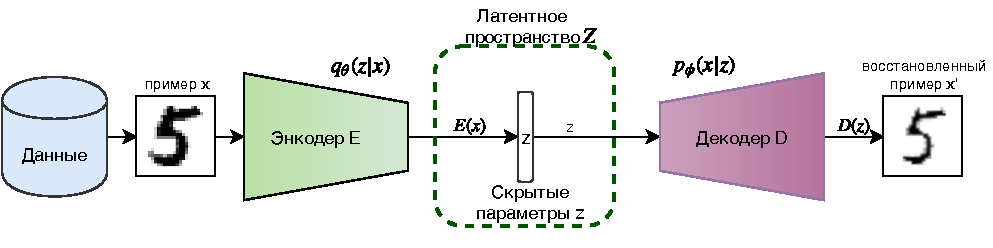
\includegraphics[width=0.8\textwidth]{img/vae}
				\caption{Схема работы вариационных автоэнкодеров (VAE)}
				\label{fig:vae}
			\end{figure}
			\noindent
			Задача автокодировщика состоит в минимизации разницы между исходным изображением $x$ и восстановленным $x'$.
			Для этого вводится функцию потерь $\mathcal{L}_{AE}$, характеризующая потери при неправильном принятии решений:
			\begin{equation} \label{eq:ae}
				\mathcal{L}_{AE}(x,x') = \|x - x'\|^{2}
			\end{equation}
			Основная проблема автоэнкодеров заключается в том, что скрытое пространство, может не быть непрерывным.
			Из-за чего не получается произвести интерполяцию, и как следствие, их область применения ограничивается.
			Эту проблему способны решить вариационные приближения.
	
		\subsection{Вариационные автокодироващики (VAE)}		

			\textbf{Вариационный автоэнкодер} (VAE) отличается от автоэнкодера непрерывностью латентного пространства
			и предположениями накладываемыми на распределение данных.
			Пусть выбор тренировочных данных $x$ находится в некоторой условной зависимости $p(x|z)$ от переменных скрытого пространства $z$.
			Кодировщик на вход получает пример $x$ и выдает вектор размерности $2d$ распределения скрытых переменных $z$, состоящий из двух векторов размерности $d$:
			вектора стандартных отклонений $\sigma$ и вектора средних значений $\mu$. 
			То есть энкодер представляет собой нейронную сеть с параметрами $\theta$ и обучается апроксимировать апостериорное распределение $q_{\theta}(z|x)$.
			Декодировщик тоже является нейронной сетью с параметрами $\phi$ и старается из вектора размерности $2d$ скрытых переменных $z$ получить объект из вариационного распределения над $x$: $p_{\phi}(x|z)$.
			На рисунке \ref{fig:vae} представлена верхнеуровневая схема модели вариационных автоэнкодеров.

			Задачей вариационных автоэнкодеров является задача оптимизации \eqref{eq:vae}.
			Необходимо так подобрать параметры $\theta$ в $q_{\theta}(z|x)$, чтобы максимально точно приблизить $p(z|x)$:
			\begin{equation} \label{eq:vae}
				\arg\min_{\theta} \mathbb{KL}(q_{\theta}(z|x)\|p(z|x)), \text { где }
			\end{equation}
			\begin{equation*}
				\mathbb{KL}(q_{\theta}(z|x)\|p(z|x)) = \mathbb{E}_q[\log q_{\theta}(z|x)] - \mathbb{E}_q[\log p(x,z)] + \log p(x)
			\end{equation*}
			$\mathbb{KL}$ -- расстояние Кульбака-Лейблера - мера удаленности двух распределений.
			\\\\ 
			Так или иначе, методы реализующие перенос изображений опираются на сети GAN, VAE или их модификации.
			Рассмотрим следующие алгоритмы с позиции решения предложенной задачи изменения времени суток на изображении.
			Будем рассматривать, уже введенные в формальном определении, домены изображений \(X_{1}\) и \(X_{2}\), соответсвующие разному времени суток (глава \ref{intro_problem}).
			\\Пусть изображения \(x_{1},x_{2}: x_{1} \in X_{1}, x_{2} \in X_{2}\)
		
		\subsection{Методы использующие обучение с учителем}
		
			\textbf{Обучение с учителем} (англ. \textit{supervised learning}) -- способ машинного обучения, в ходе которого входные данные соотносятся с выходными до начала обучения.
			Обучение происходит на заготовленных парах объектов (\(x_{1},x_{2}\)), называемыми ''стимул-реакция'', которые находятся в доменах в некотором совместном распределении \(P_{X_{1},X_{2}}(x_{1},x_{2})\)\footnote{
				\textbf{Совместное распределение} -- это распределение совместных исходов образованных из нескольких случайных величин.
			}.
			Задача метода -- построить функцию внутренней зависимости между примерами, которая затем будет отображать входные изображения желаемым образом.

			Успешными примерами применения этого способа для решения задач переноса изображения можно считать эти работы \cite{BicycleGAN, pix2pix}.

			\subsubsection{Перенос изображение и условные генеративные сети (cGAN)}
				Метод представленный на международной конференции компьютерного зрения (CVPR) в 2017 году
				исследовательской группой из университета Беркли под именем pix2pix \cite{pix2pix}
				использует для переноса изображений обучение с учителем и условные генеративно состязательные нейронные сети.

				Условные GAN являются модификацией над стандартными GAN.
				От обычных генеративных сетей \eqref{eq:gan}, cGAN отличаются добавочным вектором информации $y$ для генератора \(G(z|y) = x'\) и дискриминатора \(D(X|y)\).
				Вектор $y$ может содержать любую уточняющую информацию, например он может содержать метки объектов на изображении,
				в случае c pix2pix, $y$ -- это добавочное входное изображение, видимое генератору и дискриминатору.

				\begin{figure}[ht]
					\centering
					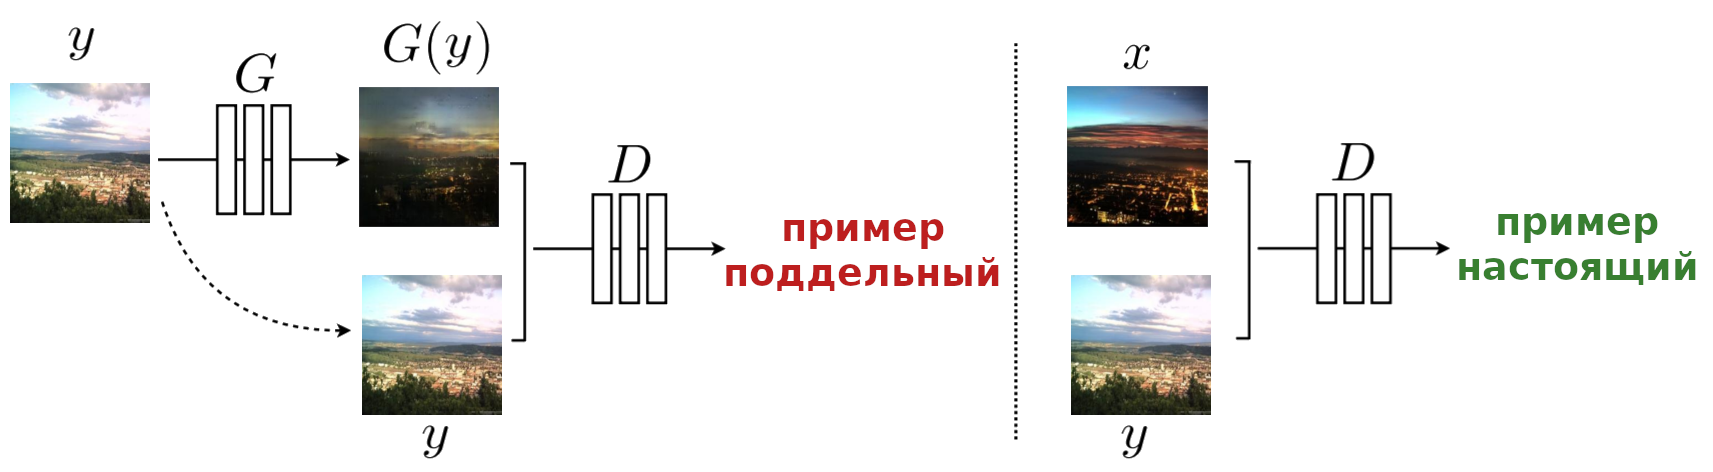
\includegraphics[width=0.9\textwidth]{img/cgan}
					\caption{Схема работы условно генеративно состязательной сети (cGAN)}{
						$x$ -- \emph{настоящее изображение ночи, соответсвующее} $y$
					}
					\label{fig:cgan}
				\end{figure}
				\noindent
				Выше на рис. \ref{fig:cgan} приведена общая схема работы модели pix2pix.
				В качестве функции потерь была взята соовокупность функций потерь: генеративной сети \eqref{eq:gan} в случае с cGAN и $\mathcal{L}_1$.
				Сеть решает следующую задачу оптимизации:
				\begin{equation}\label{eq:cgan}
					\arg\min_{G}\max_{D}\mathcal{L}_{cGAN}(D,G) + \lambda \mathcal{L}_1(G), \text{ где }
				\end{equation}
				\begin{equation*}
						\mathcal{L}_{cGAN}(D,G) = \mathbb{E}_{x}[\log{D(x)}] + \mathbb{E}_{y,z}[\log (1 - D(G(z,y)))],\;
						\mathcal{L}_1(G) = \sum_{i=1}^{n}(x - G(z,y))^2
				\end{equation*}
				$\lambda$ -- параметр, контролирующий вклад $\mathcal{L}_1$.
				При $\lambda = 0$ получаются более четкие изображения, но подверженные артефактам,
				при больших значениях параметра, будут получаться менее четкие, размытые изображения, но с визуально уменьшенным количеством артефактов \cite{pix2pix}.
				Модель обучалась на датасете\footnote{ \textbf{Датасет} (англ. \textit{dataset}) -- то же, что и набор данных} \cite{data:paired_night2day}
				парных фотографиях (с одинаковых ракурсов) сделанных с уличных вебкамер в разрешении 256x256px в разное время суток.
				После проведения серии экспериментов стало ясно, что из-за большого числа артефактов и размытости данную модель в своей задаче использовать не получится.
				Это происходит из-за того, что в датасете \cite{data:paired_night2day} используется всего 101 уникальная пара,
				а на данных, немного отличными от обучающей выборки, точность модели падает.
				Резльтаты работы метода на рис. \ref{fig:pix2pix_results}.
				
				\begin{figure}[ht]
					\centering
					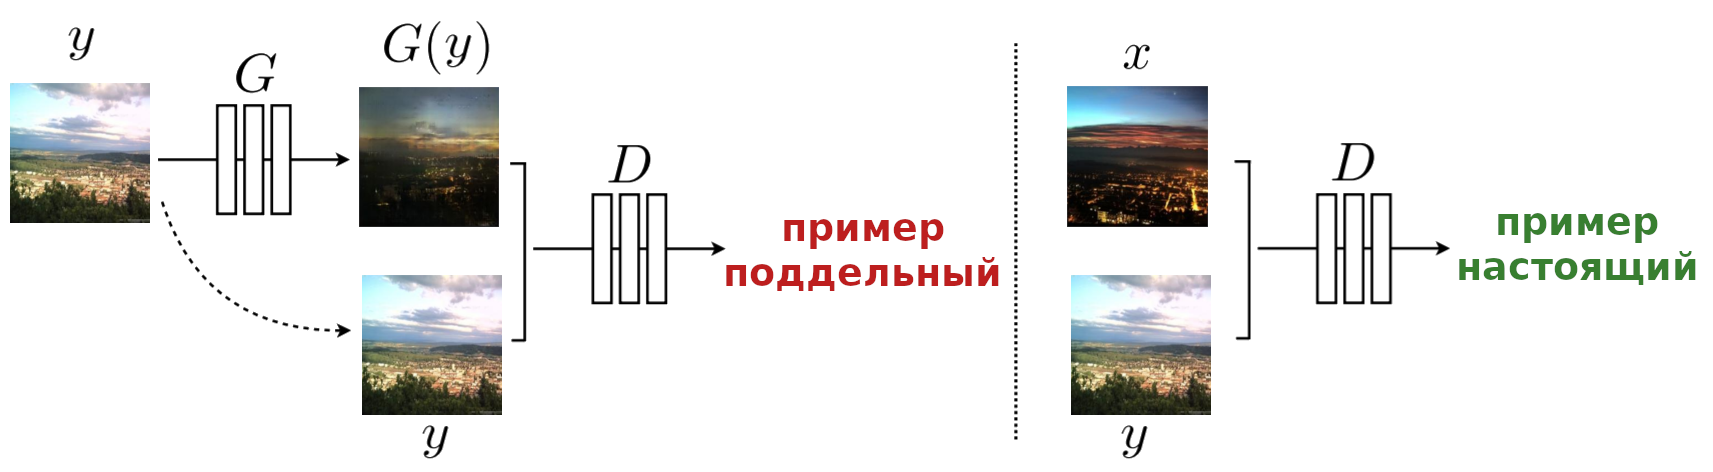
\includegraphics[width=0.9\textwidth]{img/cgan}
					\caption{Схема работы условно генеративно состязательной сети (cGAN)}{
						$x$ -- \emph{настоящее изображение ночи, соответсвующее} $y$
					}
					\label{fig:pix2pix_results}
				\end{figure}
				
				Существенным и основным недостатком медотов, использующих обучение с учителем, является необходимость хранить объекты доменов по парам.
				Это сказывается на сложности поиска и сбора тренировочных данных, для применения их на практике.
				С другой стороны, методы без учителя, лишены этого недостатка, и данные можно получать фактически ''из воздуха''.
				
				
		\subsection{Методы использующие обучение без учителя}
			\textbf{Обучение без учителя} (англ. \textit{unsupervised learning}) -- совокупность задач машинного обучения, решаемых на неразмеченных данных.
			В отличие от обучения с учителем, где тренировочные данные находятся в совместном распределении \(P_{X_{1},X_{2}}(x_{1},x_{2})\), в методах без вмешательства учителя требуется
			найти априорное распределение, выбирая данные (\(x_{1},x_{2}\)) из доменов с частным распределением \(P_{X_{1}}(x_{1})\) и  \(P_{X_{2}}(x_{2})\)\footnote{
				\textbf{Частное распределение} -- это распределение вероятности компонент некоторого множества, без зависимости между компонентами.
			}.

			К наиболее интересным работам, использующим этот метод, можно отнести \cite{UNIT,MUNIT,CycleGAN}.

		% \subsection{Выводы}
			
% \section{Исследование и построение решения задачи}

% \section{Описание практической части}
% \textit{датасетов}\footnote{
% 				\textbf{Датасет} (англ. \textit{dataset}) -- то же, что и набор данных.
% 				} 
% \section{Заключение}

\newpage

\begin{thebibliography}{00}

	
	\bibitem{i2ipapers}
	\textbf{Supervised and Unsupervised Image Translation} --
	\href{https://github.com/lzhbrian/image-to-image-papers}{A collection of image to image papers with code},
	2019.

	\bibitem{style_transfer}
	\textbf{J.Johnson, A.Alahi, L.Fei-Fei}.
	\emph{Perceptual Losses for Real-Time Style Transfer and Super-Resolution}.
	Department of Computer Science, Stanford University,
	March 2016.

	\bibitem{color_transfer}
	\textbf{R.Zhang, J.-Y.Zhu, P.Isola, X.Geng, A.S.Lin, T.Yu, A.A.Efros}.
	\emph{Real-Time User-Guided Image Colorization with Learned Deep Priors}.
	University of California, Berkeley,
	May 2017.

	\bibitem{CycleGAN}
	\textbf{J.-Y.Zhu, T.Park, P.Isola, A.A.Efros}.
	\emph{Unpaired Image-to-Image Translation using Cycle-Consistent Adversarial Networks}.
	Berkeley AI Research (BAIR) laboratory, UC Berkeley,
	March 2017.

	\bibitem{pix2pix}
	\textbf{P.Isola, J.-Y.Zhu, T.Zhou, A.A.Efros}.
	\emph{Image-to-image translation with conditional adversarial networks}.
	Berkeley AI Research (BAIR) laboratory, UC Berkeley,
	November 2016.

	\bibitem{super_resolution}
	\textbf{Y.Yuan, S.Liu, J.Zhang, Y.Zhang, C.Dong, L.Lin}
	\emph{Unsupervised Image Super-Resolution using Cycle-in-Cycle Generative Adversarial Networks}
	Guangdong Key Laboratory of Intelligent Information Processing, Shenzhen University,
	Graduate School at Shenzhen, Department of Automation, Tsinghua University,
	September 2018.

	\bibitem{UNIT}
	\textbf{M.-Y.Liu, T.Breuel, J.Kautz}.
	\emph{Unsupervised Image-to-Image Translation Networks}.
	NVIDIA Corporation,
	March 2017.
	
	\bibitem{MUNIT}
	\textbf{X.Huang, M.-Y.Liu, S.Belongie, J.Kautz}.
	\emph{Multimodal Unsupervised Image-to-Image Translation}.
	Cornell University, NVIDIA Corporation,
	April 2018.

	\bibitem{BicycleGAN}
	\textbf{J.-Y.Zhu, R.Zhang, D.Pathak, A.A.Efros}.
	\emph{Toward Multimodal Image-to-Image Translation}.
	Berkeley AI Research, UC Berkeley, Adobe Research,
	November 2017.

	\bibitem{EG-UNIT}
	\textbf{L.Ma, X.Jia, S.Georgoulis, T.Tuytelaars, L.V.Gool}.
	\emph{Exemplar Guided Unsupervised Image-to-Image Translation}.
	Berkeley AI Research, UC Berkeley, Adobe Research,
	March 2019.
	
	\bibitem{Deep_Learning}
	\textbf{С.Николенко, А.Кадурин, Е.Архангельская}.
	\emph{Глубокое обучение}.
	СПб.: Питер, 
	2018.

	\bibitem{ml_lang}
	\textbf{The State of the Octoverse: machine learning} --
	\href{https://github.blog/2019-01-24-the-state-of-the-octoverse-machine-learning/}{GitHub: Report},
	January 2019.

	\bibitem{data:paired_night2day}
	\textbf{Dateset: Paired WebCam Night2Day} -- 
	\href{http://efrosgans.eecs.berkeley.edu/pix2pix/datasets/}{UC Berkley, pix2pix and BycicleGAN projects}

\end{thebibliography}

\end{document}